\documentclass[11pt]{report}
\usepackage[utf8]{inputenc}
\usepackage[margin=2.0cm]{geometry}
\usepackage{fancyhdr}
\usepackage{xcolor}
\usepackage{minted}
\usepackage{graphicx}
\usepackage[parfill]{parskip}

\title{Digital Engineering\\Lab 3}
\author{Y3890959\\Y3878784}
\date{7th February 2023}

\pagestyle{fancy}
\fancyhead{}
\setlength{\headheight}{14pt}
\fancyhead[L]{Lab 3}
\fancyhead[R]{Y3890959, Y3878784}
\fancyfoot{}
\fancyfoot[L]{Digital Engineering}
\fancyfoot[R]{\thepage}

\makeatletter
\let\ps@plain\ps@fancy 
\makeatother

\setminted {
    fontsize=\footnotesize,
    frame=single,
}

\begin{document}

\maketitle

\chapter*{Task A: Pipelining}

\section*{2.1.1 Behaviour Simulation}
\subsection*{Waveform 1: Global Initialisation/Reset}
\begin{figure}[H]
    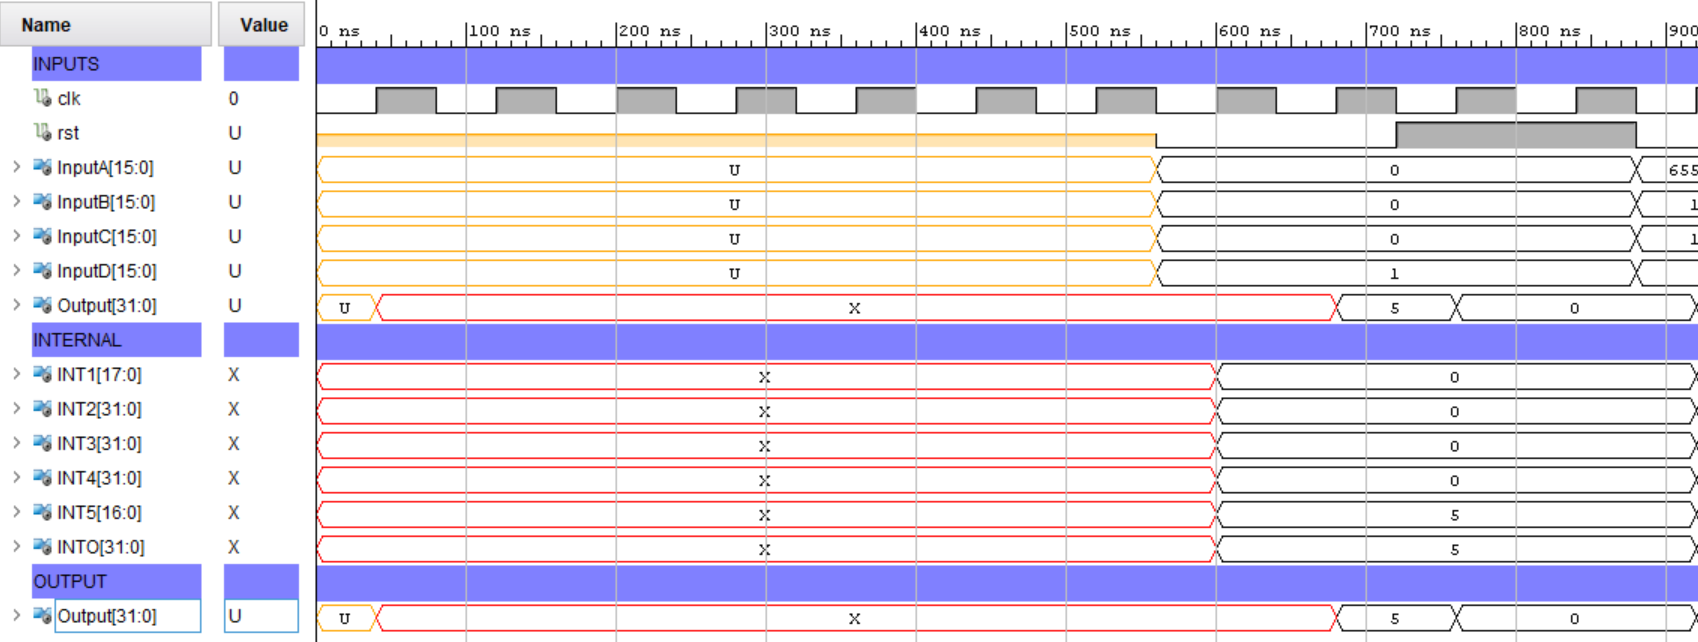
\includegraphics[width=\columnwidth]{Reports/Lab3/Assets/2.1.1_waveform-initial-reset.png}
\end{figure}

\subsection*{Waveform 2: Test Sequence}
\begin{figure}[H]
    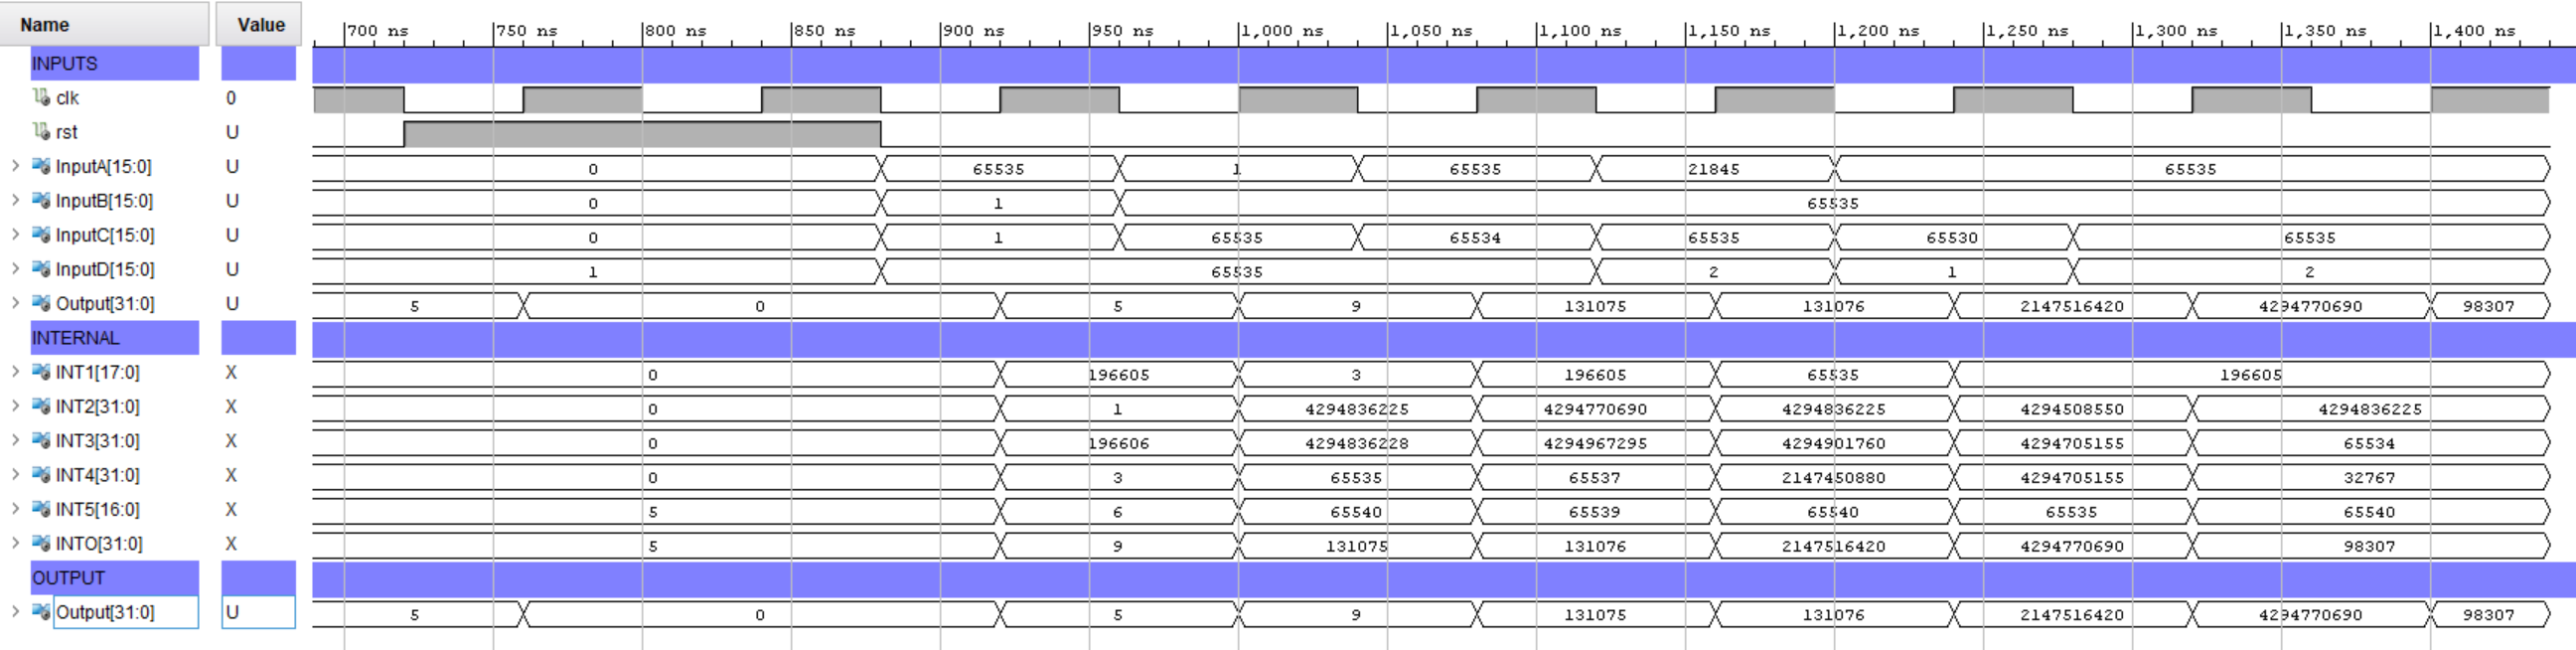
\includegraphics[width=\columnwidth]{Reports/Lab3/Assets/2.1.1_waveform-test-sequence.png}
\end{figure}

\subsection*{Console Output}
\begin{figure}[H]
    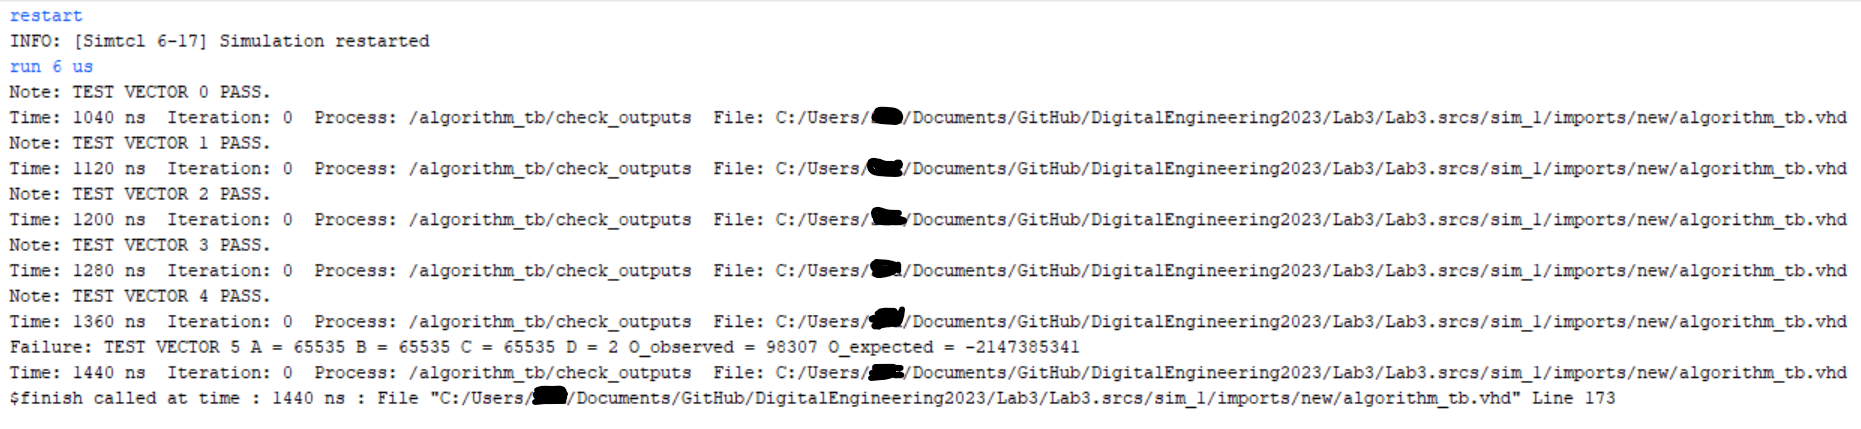
\includegraphics[width=\columnwidth]{Reports/Lab3/Assets/2.1.1_console.png}
\end{figure}

\section*{2.1.2 Design Runs}
\begin{figure}[H]
    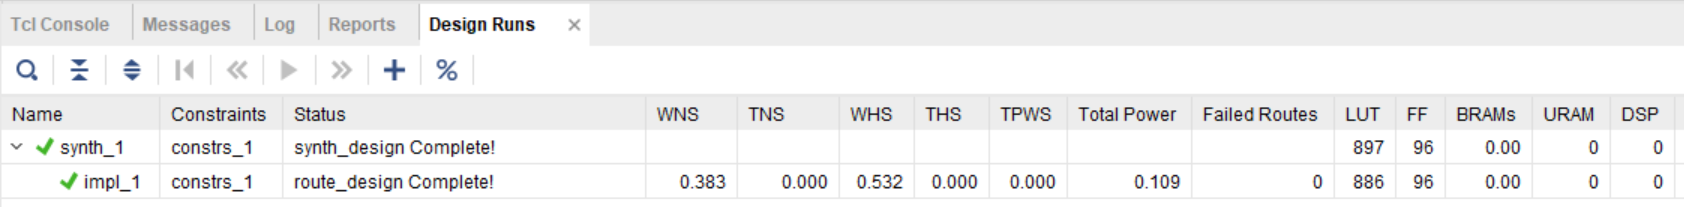
\includegraphics[width=\columnwidth]{Reports/Lab3/Assets/2.1.2_design-runs.png}
\end{figure}
The best period where the constraints are met is at 107ns with a WNS of 0.383ns. The tools fail with a 106ns constraint. The fastest frequency at which this design can run, taking into account the WNS value, is 9.379MHz.


\section*{2.1.3 Post-Route Timing Report: Max Delay Path}
\begin{figure}[H]
    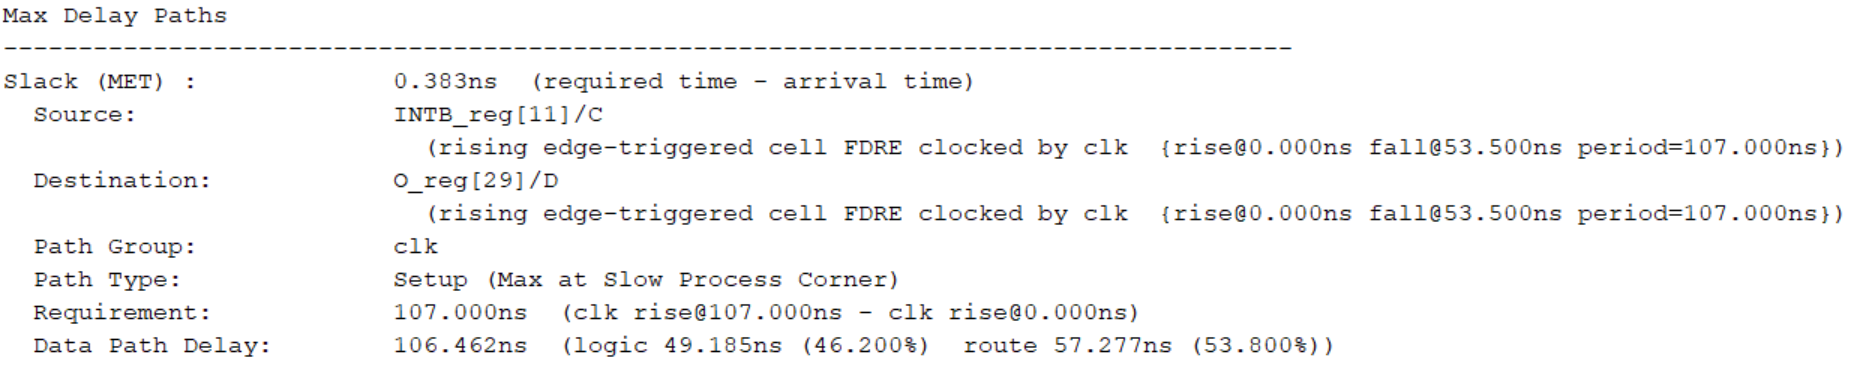
\includegraphics[width=\columnwidth]{Reports/Lab3/Assets/2.1.3_max-delay-path.png}
\end{figure}

\section*{2.1.4 Pipeline 1 Behavioural Simulation}
\subsection*{Waveform 1: Global Initialisation/Reset}
\begin{figure}[H]
    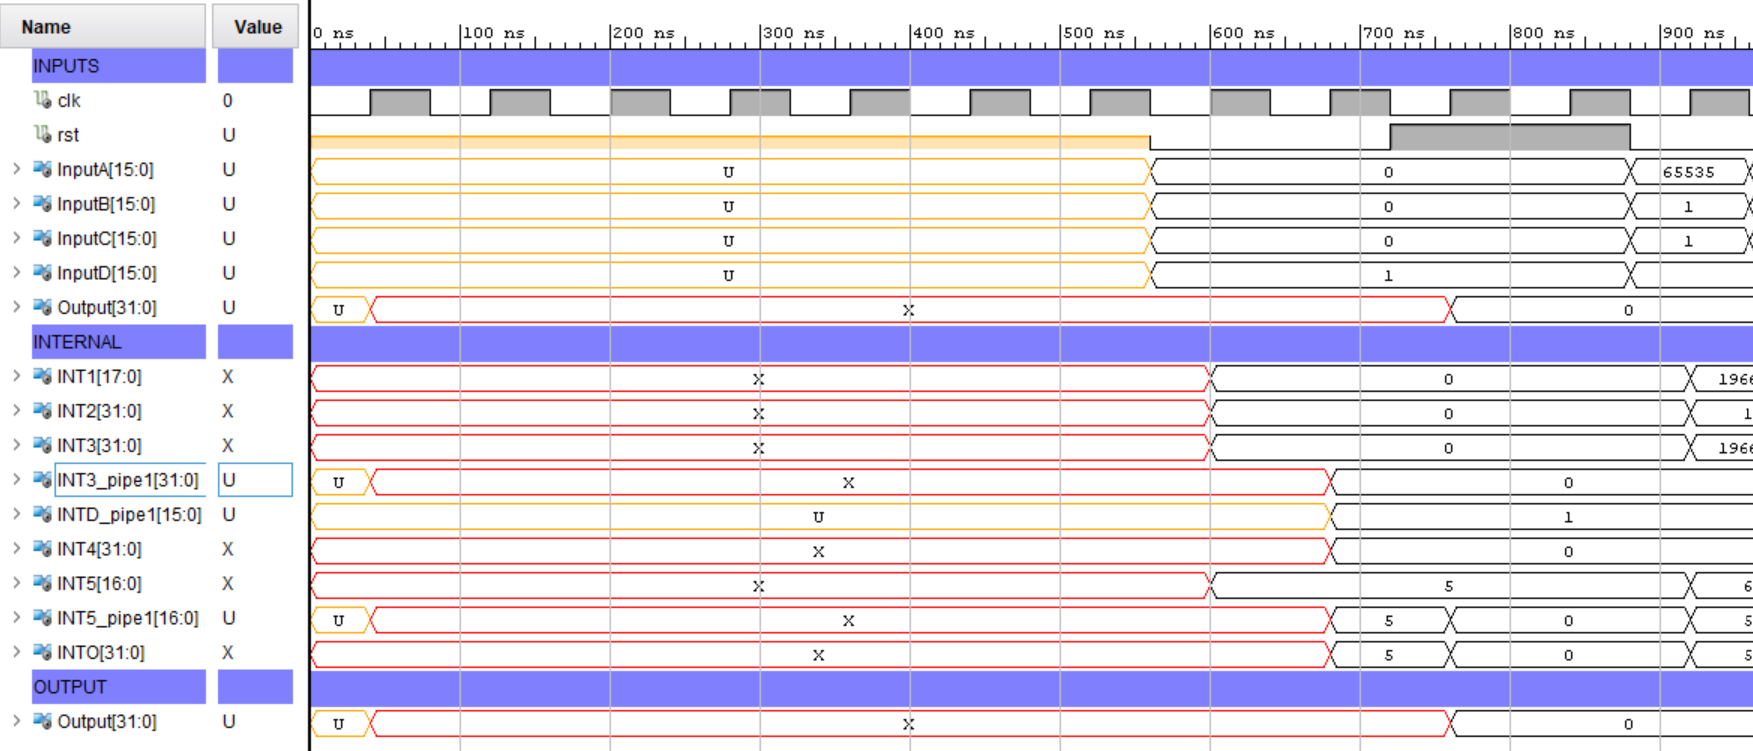
\includegraphics[width=\columnwidth]{Reports/Lab3/Assets/2.1.4_waveform-initial-reset.png}
\end{figure}

\subsection*{Waveform 2: Test Sequence}
\begin{figure}[H]
    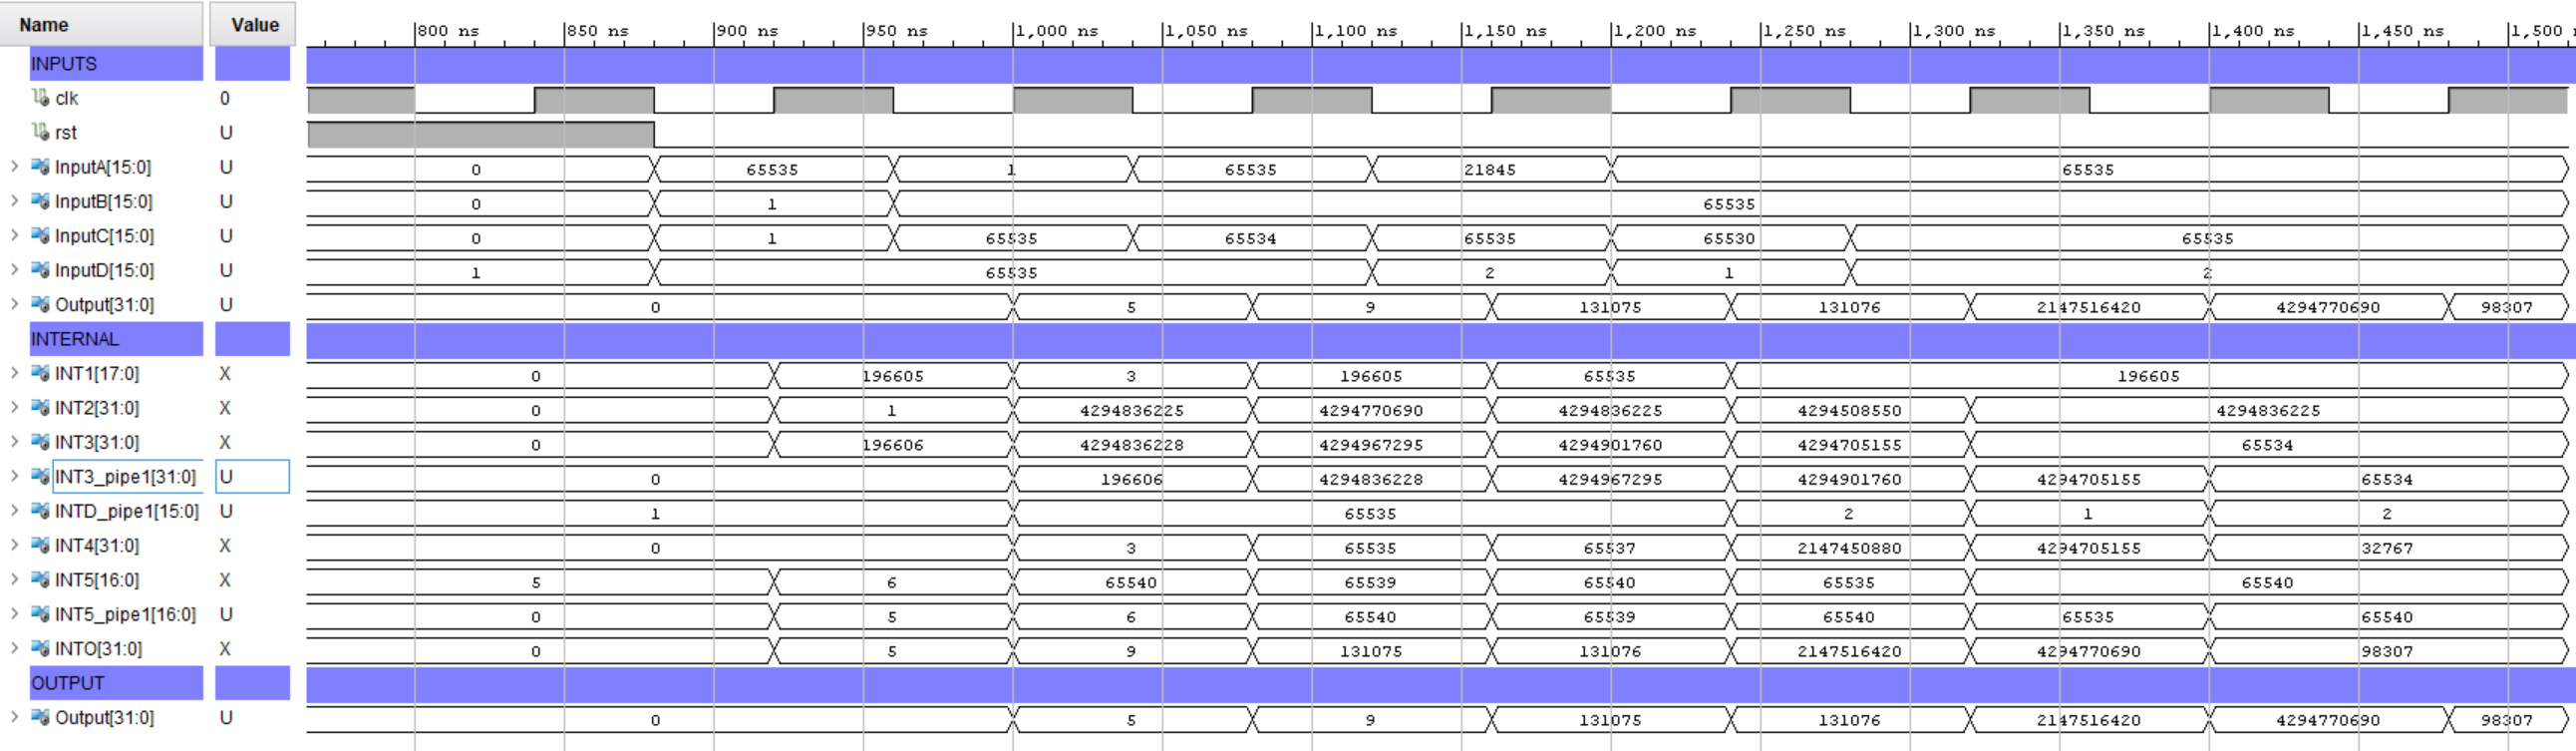
\includegraphics[width=\columnwidth]{Reports/Lab3/Assets/2.1.4_waveform-test-sequence.png}
\end{figure}

\subsection*{Console}
\begin{figure}[H]
    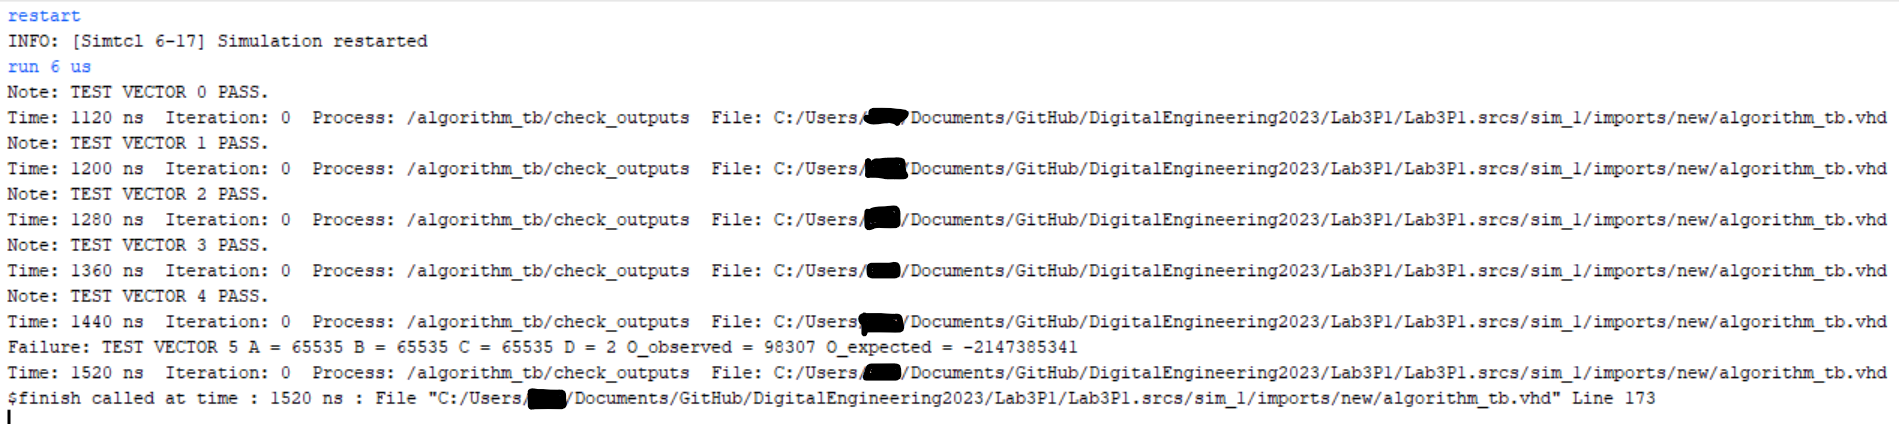
\includegraphics[width=\columnwidth]{Reports/Lab3/Assets/2.1.4_console.png}
\end{figure}

\section*{2.1.5 Design Runs}
\begin{figure}[H]
    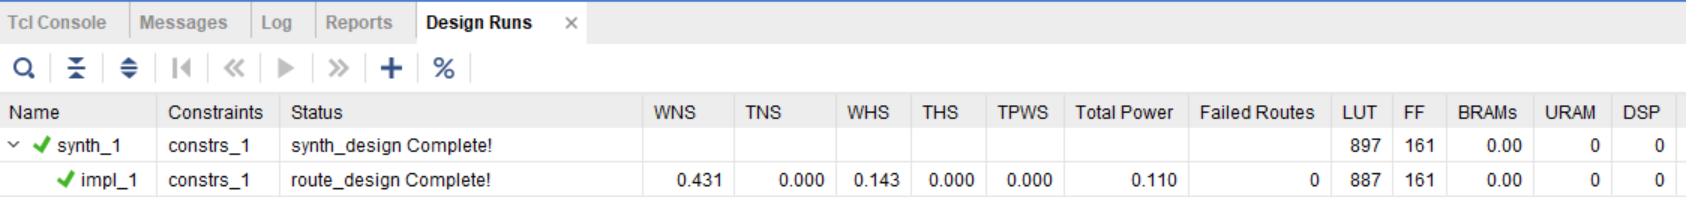
\includegraphics[width=\columnwidth]{Reports/Lab3/Assets/2.1.5_design-runs.png}
\end{figure}
The best period where the constraints are met is at 96ns with a WNS of 0.431ns. The tools fail with a 95ns constraint. The fastest frequency at which this design can run, taking into account the WNS value, is 10.37MHz.

\section*{2.1.6 Post-Route Timing Report: Max Delay Path}
\begin{figure}[H]
    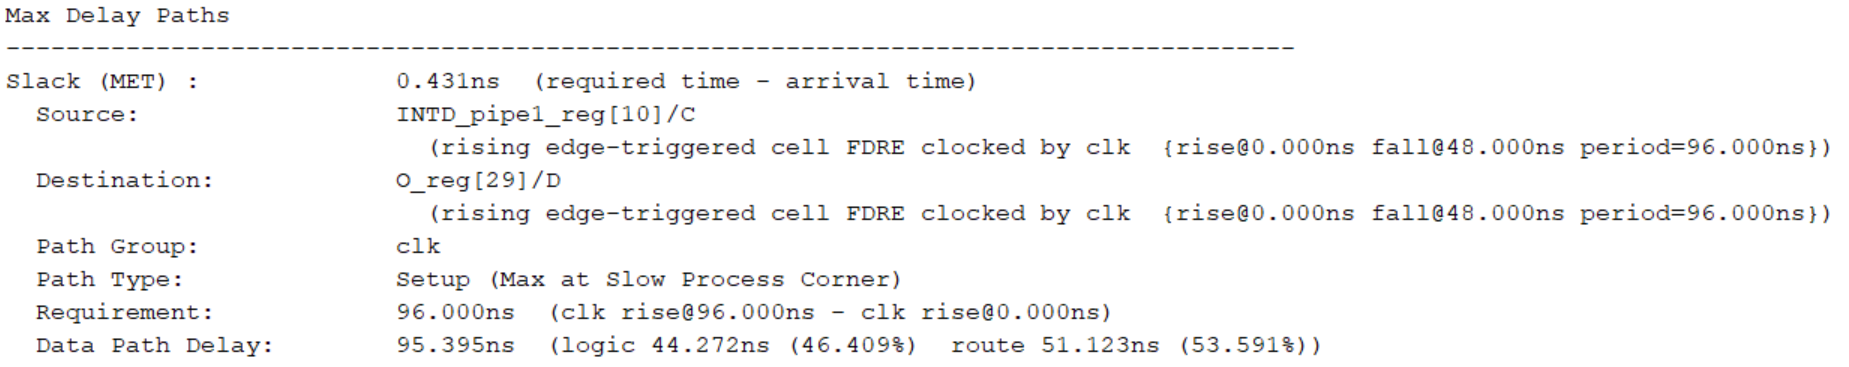
\includegraphics[width=\columnwidth]{Reports/Lab3/Assets/2.1.6_max-delay-path.png}
\end{figure}
Before the pipeline was added, the critical path was detected between INTB\_reg and O\_reg. Now, we've reduced the effect of that by adding a pipeline. Now the detected critical path is between INTD\_pipe1\_reg and O\_reg. The critical path consists of the division and the addition operation, This does in fact increase the max clock period that the circuit can support as per the theory.

\end{document}
